\section{Study Design}

We designed a controlled study of two protocol-design axes in inference-time Self-Refinement: which refinement roles are included and whether those roles are externalized across calls or specified within one call.
For each model and task, every condition started from the same self-generated Initial Candidate, and no model call received execution feedback.
This section defines the Research Questions, protocol stages and compositions, evaluated models and benchmarks, and experimental procedure.

\subsection{Research Questions}

\researchquestion{RQ1}{How does the stage composition of Self-Refinement affect final code correctness, and how is that effect explained by repairs of initially incorrect candidates and regressions of initially correct candidates?}
An explicit Critique or Revision Plan may structure refinement, but an added stage can also alter a candidate that was already correct.
We therefore compare Direct Generation with revision alone, Critique followed by Revision, and Critique followed by Planning and Revision, while jointly interpreting final correctness through Repair, Correct-to-Incorrect Regression, Functional Preservation, and Unrepaired Failure.

\researchquestion{RQ2}{How does the value of Decision-Conditioned Refinement vary across model-benchmark combinations with different initial pass rates?}
A Decision stage can preserve a candidate exactly and avoid unnecessary refinement, but an incorrect preservation decision can also forgo a possible repair.
We compare each always-refine path with its Decision-conditioned counterpart and relate the resulting prevented regressions, missed repairs, correctness differences, and token savings to the observed Initial Pass Rate of each model-benchmark combination.

\researchquestion{RQ3}{How does realizing refinement roles within one model call versus externalizing them across multiple calls affect correctness and preservation?}
Separate calls make intermediate artifacts and exact selection observable, whereas one call avoids reintroducing those artifacts as later inputs but does not enforce the same boundaries.
We compare matched single-call and separate-call realizations of the same role sequences using the exact same Initial Candidates and evaluate final correctness, functional transitions, candidate preservation, and agreement between an integrated Decision label and the code emitted with it.

\researchquestion{RQ4}{Do the correctness effects of alternative refinement protocols justify their token costs?}
Externalized stages add calls and intermediate-input tokens, while single-call protocols reduce call count but may change correctness or preservation.
We compare correctness with end-to-end Protocol-Implied Token Cost across the complete protocol panel, including the calls avoided by a \texttt{PRESERVE} Decision.

\subsection{Self-Refinement Protocols}

For each model-task pair, Direct Generation produced one Initial Candidate from the Task Specification.
The candidate was stored once and reused as the exact input to every refinement variant, so differences between variants did not arise from different initial generations.
We refer to this control as the Shared-Initial Design.
Benchmark execution was reserved for evaluation and provided no feedback to the model.

We describe refinement using four role labels: Refinement-Need Decision (\texttt{D}), Critique Generation (\texttt{C}), Revision Planning (\texttt{P}), and Code Revision (\texttt{R}).
In the separate-call conditions, each label denotes an observable prompt and model call whose output was stored before a downstream call.
In the single-call conditions, the labels instead denote roles ordered within one prompt and do not establish that the model's unobserved reasoning followed those roles internally.

\subsubsection{Refinement Stages}

Refinement-Need Decision (\texttt{D}) receives only the Task Specification and exact Initial Candidate and returns \texttt{PRESERVE} or \texttt{REFINE}.
It does not generate a Critique, Plan, or revised code and is not provided to any Critique, Planning, or Revision prompt.
Its function in a separate-call protocol is exact selection: \texttt{PRESERVE} selects the stored Initial Candidate, whereas \texttt{REFINE} selects the candidate from a matched refinement path.

Critique Generation (\texttt{C}) receives the Task Specification and Initial Candidate and diagnoses whether the candidate has a functional problem.
When a problem is found, the Critique identifies its root cause and relevant code location; otherwise, it records a no-problem conclusion.
The call is not asked to produce a completed Revision Plan or a revised solution, and we do not assign an independent correctness label to its text artifact.

Revision Planning (\texttt{P}) receives the Task Specification, Initial Candidate, and stored Critique.
It translates the Critique into concrete minimal changes and preservation constraints, or records that no change is needed when the Critique found no problem.
Planning is not instructed to conduct a second independent review and does not produce the complete revised program.
We use Planning only after Critique because a plan produced without a prior diagnosis would combine problem identification and edit planning rather than isolate the same translation role.

Code Revision (\texttt{R}) is the only separate-call Refinement Stage that produces executable code.
Direct Revision receives the Task Specification and Initial Candidate and must determine for itself whether a functional change is needed.
Critique-Conditioned Revision instead acts on the stored Critique, whereas Plan-Conditioned Revision acts on the stored Plan and does not receive the Critique text directly.
The conditioned Revision prompts request an exact reproduction of the Initial Candidate when their supplied artifact indicates that no change is needed.
Every Revision response must contain exactly one complete fenced Python block, and no Revision prompt receives a Decision or execution feedback.

\subsubsection{Separate-Call Protocols for RQ1 and RQ2}

The three Always-Refine Protocols are named by the execution order of their separately invoked stages.
Direct Revision (\texttt{R}) performs one Revision call without an upstream artifact.
Critique-Conditioned Revision (\texttt{CR}) executes Critique Generation and then provides the stored Critique to a separate Revision call.
Critique-and-Plan-Conditioned Revision (\texttt{CPR}) executes Critique Generation, translates the stored Critique in a separate Planning call, and provides only the resulting Plan to a separate Revision call.
The same Critique artifact is reused by \texttt{CR} and Planning, so their difference does not include independently sampled Critiques.
RQ1 compares Direct Generation with \texttt{R}, \texttt{R} with \texttt{CR}, and \texttt{CR} with \texttt{CPR} to measure complete Stage-Composition effects together with their Repair and Regression balance.

Combining \texttt{D} with \texttt{R} yields Decision-Conditioned Direct Revision (\texttt{DR}).
Its combinations with \texttt{CR} and \texttt{CPR} yield Decision-Conditioned \texttt{CR} (\texttt{DCR}) and Decision-Conditioned \texttt{CPR} (\texttt{DCPR}), respectively.
No additional Revision call is made to construct these outcomes.
If the Decision is \texttt{PRESERVE}, the protocol selects the exact Initial Candidate; if it is \texttt{REFINE}, it selects the matched Always-Refine candidate.
RQ2 compares each Decision-conditioned protocol with its Always-Refine counterpart to quantify prevented regressions, missed repairs, and conditionally avoided calls across model-benchmark combinations.

\subsubsection{Single-Call Protocols for RQ3}

The Single-Call Role Protocols specify multiple roles in one prompt but make one model call from the Task Specification and exact Initial Candidate.
Single-Call Critique and Revision (\texttt{SC-CR}) orders the \texttt{C} and \texttt{R} roles, and Single-Call Critique, Planning, and Revision (\texttt{SC-CPR}) orders \texttt{C}, \texttt{P}, and \texttt{R}; both responses require only the final code.
Single-Call Decision and Revision (\texttt{SC-DR}), Single-Call Decision, Critique, and Revision (\texttt{SC-DCR}), and Single-Call Decision, Critique, Planning, and Revision (\texttt{SC-DCPR}) additionally require an exact first-line Decision label in the same response as the final code.
We do not define a separate \texttt{SC-R} condition because \texttt{R} is already a one-call protocol with the same role scope.

For the primary \texttt{SC-D*} outcome, the Final Candidate is the code emitted by that call regardless of its Decision label.
The label and code are parsed independently, so a valid code candidate remains available even if its label is invalid, and a valid label remains recorded when the code is malformed.
Selecting the exact Initial Candidate for \texttt{PRESERVE} and the emitted code for \texttt{REFINE} forms a supplementary label-enforced outcome without another model call.
RQ3 compares \texttt{CR} with \texttt{SC-CR}, \texttt{CPR} with \texttt{SC-CPR}, and each of \texttt{DR}, \texttt{DCR}, and \texttt{DCPR} with its matched \texttt{SC-D*} protocol.
These contrasts estimate the end-to-end effect of prompt-and-call topology, not the independent semantic accuracy of an unobserved internal Critique, Plan, or Decision process.
RQ4 places Direct Generation and all 11 refinement outcomes in a common correctness-cost comparison.

Figure~\ref{fig:protocol-overview} summarizes the separate-call compositions used for RQ1 and RQ2 and their single-call counterparts used for RQ3.

\begin{figure}[H]
\centering
\resizebox{0.98\columnwidth}{!}{%
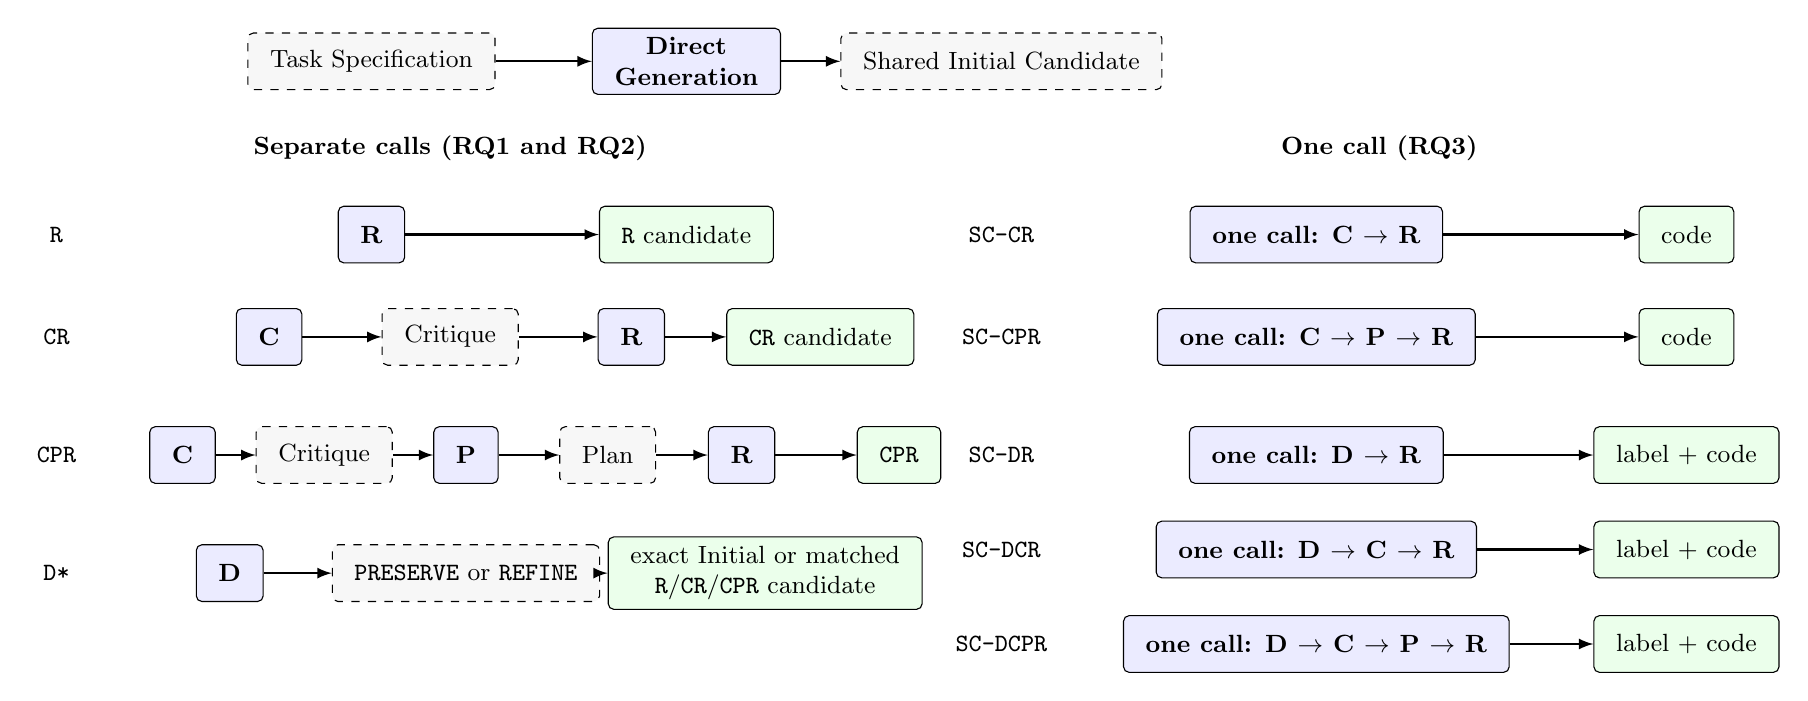
\begin{tikzpicture}[
    stage/.style={draw, rounded corners=2pt, fill=blue!8, align=center, minimum height=0.72cm, inner xsep=8pt, font=\small\bfseries},
    artifact/.style={draw, dashed, rounded corners=2pt, fill=black!3, align=center, minimum height=0.72cm, inner xsep=8pt, font=\small},
    outcome/.style={draw, rounded corners=2pt, fill=green!8, align=center, minimum height=0.72cm, inner xsep=8pt, font=\small},
    flow/.style={->, >=latex, thick},
    label/.style={font=\small\ttfamily\bfseries}
]
\node[artifact] (task) at (4.0,5.0) {Task Specification};
\node[stage] (generation) at (8.0,5.0) {Direct\\Generation};
\node[artifact] (initial) at (12.0,5.0) {Shared Initial Candidate};
\draw[flow] (task) -- (generation);
\draw[flow] (generation) -- (initial);

\node at (5.0,3.9) {\small\bfseries Separate calls (RQ1 and RQ2)};
\node at (16.8,3.9) {\small\bfseries One call (RQ3)};

\node[label] at (0.0,2.8) {R};
\node[stage] (r-direct) at (4.0,2.8) {R};
\node[outcome] (r-candidate) at (8.0,2.8) {\texttt{R} candidate};
\draw[flow] (r-direct) -- (r-candidate);

\node[label] at (0.0,1.5) {CR};
\node[stage] (critique) at (2.7,1.5) {C};
\node[artifact] (critique-artifact) at (5.0,1.5) {Critique};
\node[stage] (r-critique) at (7.3,1.5) {R};
\node[outcome] (cr-candidate) at (9.7,1.5) {\texttt{CR} candidate};
\draw[flow] (critique) -- (critique-artifact);
\draw[flow] (critique-artifact) -- (r-critique);
\draw[flow] (r-critique) -- (cr-candidate);

\node[label] at (0.0,0.0) {CPR};
\node[stage] (critique-cpr) at (1.6,0.0) {C};
\node[artifact] (critique-cpr-artifact) at (3.4,0.0) {Critique};
\node[stage] (planning) at (5.2,0.0) {P};
\node[artifact] (plan-artifact) at (7.0,0.0) {Plan};
\node[stage] (r-plan) at (8.7,0.0) {R};
\node[outcome] (cpr-candidate) at (10.7,0.0) {\texttt{CPR}};
\draw[flow] (critique-cpr) -- (critique-cpr-artifact);
\draw[flow] (critique-cpr-artifact) -- (planning);
\draw[flow] (planning) -- (plan-artifact);
\draw[flow] (plan-artifact) -- (r-plan);
\draw[flow] (r-plan) -- (cpr-candidate);

\node[label] at (0.0,-1.5) {D*};
\node[stage] (decision) at (2.2,-1.5) {D};
\node[artifact] (decision-artifact) at (5.2,-1.5) {\texttt{PRESERVE} or \texttt{REFINE}};
\node[outcome] (selection) at (9.0,-1.5) {exact Initial or matched\\\texttt{R}/\texttt{CR}/\texttt{CPR} candidate};
\draw[flow] (decision) -- (decision-artifact);
\draw[flow] (decision-artifact) -- (selection);

\node[label] at (12.0,2.8) {SC-CR};
\node[stage] (sc-cr) at (16.0,2.8) {one call: C $\rightarrow$ R};
\node[outcome] (sc-cr-candidate) at (20.7,2.8) {code};
\draw[flow] (sc-cr) -- (sc-cr-candidate);

\node[label] at (12.0,1.5) {SC-CPR};
\node[stage] (sc-cpr) at (16.0,1.5) {one call: C $\rightarrow$ P $\rightarrow$ R};
\node[outcome] (sc-cpr-candidate) at (20.7,1.5) {code};
\draw[flow] (sc-cpr) -- (sc-cpr-candidate);

\node[label] at (12.0,0.0) {SC-DR};
\node[stage] (sc-dr) at (16.0,0.0) {one call: D $\rightarrow$ R};
\node[outcome] (sc-dr-candidate) at (20.7,0.0) {label + code};
\draw[flow] (sc-dr) -- (sc-dr-candidate);

\node[label] at (12.0,-1.2) {SC-DCR};
\node[stage] (sc-dcr) at (16.0,-1.2) {one call: D $\rightarrow$ C $\rightarrow$ R};
\node[outcome] (sc-dcr-candidate) at (20.7,-1.2) {label + code};
\draw[flow] (sc-dcr) -- (sc-dcr-candidate);

\node[label] at (12.0,-2.4) {SC-DCPR};
\node[stage] (sc-dcpr) at (16.0,-2.4) {one call: D $\rightarrow$ C $\rightarrow$ P $\rightarrow$ R};
\node[outcome] (sc-dcpr-candidate) at (20.7,-2.4) {label + code};
\draw[flow] (sc-dcpr) -- (sc-dcpr-candidate);
\end{tikzpicture}%
}
\caption{Overview of the Shared-Initial Design and protocol composition. Every row receives the Task Specification and exact Initial Candidate. Separate boxes in the left panel denote distinct calls and stored artifact flow; each stage sequence in the right panel is specified within one call. \texttt{D*} combines one separate Decision with each matched Always-Refine candidate to derive \texttt{DR}, \texttt{DCR}, and \texttt{DCPR}.}
\label{fig:protocol-overview}
\end{figure}
\unskip

The complete frozen prompt sets were versioned before their respective executions, and raw responses were stored before parsing.
The incremental contrasts concern complete protocols: for example, \texttt{CR} versus \texttt{R} includes the Critique call, its artifact, its downstream conditioning, and its token cost, while \texttt{CPR} versus \texttt{CR} also changes the direct input to Revision from Critique to Plan.
We therefore do not interpret either contrast as an isolated causal evaluation of Critique or Plan correctness.

\subsection{Models}

\begin{table}[H]
\caption{Open-weight models evaluated in the study and their characteristics.}
\label{tab:models}
\centering
\begingroup
\scriptsize
\renewcommand{\arraystretch}{1.12}

\begin{threeparttable}

\begin{tabularx}{0.98\columnwidth}{
    >{\raggedright\arraybackslash}p{0.28\columnwidth}
    >{\raggedright\arraybackslash}X
    >{\centering\arraybackslash}p{0.20\columnwidth}
    >{\centering\arraybackslash}p{0.16\columnwidth}
}
\toprule
\textbf{Model}\tnote{a} &
\textbf{Model category} &
\textbf{Parameters}\tnote{b} &
\textbf{Precision} \\
\midrule
Qwen2.5-Coder-7B & Code-specialized, dense & 7.6B & BF16 \\
Qwen2.5-Coder-14B & Code-specialized, dense & 14.7B & BF16 \\
DeepSeek-Coder-V2-Lite & Code-specialized, MoE & 16B / 2.4B active & BF16 \\
Devstral-Small-2-24B & Software-engineering-specialized, dense & 24B & FP8 \\
Qwen3-Coder-30B-A3B & Code-specialized, MoE & 30.5B / 3.3B active & FP8 \\
Gemma-4-31B-QAT-W4A16 & General-purpose, dense & 31B & QAT W4A16 \\
\bottomrule
\end{tabularx}

\begin{tablenotes}[flushleft]
\footnotesize
\item[a]
The exact checkpoints were
\texttt{Qwen/Qwen2.5-Coder-\allowbreak 7B-Instruct},
\texttt{Qwen/Qwen2.5-Coder-\allowbreak 14B-Instruct},
\texttt{deepseek-ai/DeepSeek-Coder-\allowbreak V2-Lite-Instruct},
\texttt{mistralai/Devstral-Small-\allowbreak 2-24B-Instruct-2512},
\texttt{Qwen/Qwen3-Coder-\allowbreak 30B-A3B-Instruct-FP8}, and
\texttt{google/gemma-4-\allowbreak 31B-it-qat-w4a16-ct}.
\item[b]
For mixture-of-experts models, total and active parameter counts are shown.
\end{tablenotes}

\end{threeparttable}
\endgroup
\end{table}
\unskip

We selected six publicly available checkpoints that could be served within the same two-GPU workstation budget while covering multiple model families, parameter scales, and dense and mixture-of-experts architectures.
The panel consists primarily of code-specialized models and includes Gemma 4 as a general-purpose control.
The two Qwen2.5 models provide a within-family scale comparison, while DeepSeek-Coder-V2-Lite, Devstral, and Qwen3-Coder broaden the architecture and family coverage.
We used the official compressed checkpoints for Devstral, Qwen3-Coder, and Gemma 4 to fit the common hardware budget, and all comparisons within a model used the same checkpoint and precision.

\subsection{Benchmarks}

\begin{table}[H]
\caption{Python code-generation benchmarks evaluated in the study.}
\label{tab:benchmarks}
\centering
\begingroup
\small
\renewcommand{\arraystretch}{1.15}

\begin{threeparttable}

\begin{tabularx}{0.96\columnwidth}{
    @{\hspace{5pt}}
    >{\raggedright\arraybackslash}p{0.32\columnwidth}
    >{\centering\arraybackslash}p{0.20\columnwidth}
    >{\raggedright\arraybackslash}X
    @{\hspace{5pt}}
}
\toprule
\textbf{Benchmark} &
\textbf{Tasks analyzed} &
\textbf{Task setting} \\
\midrule
HumanEval+ v0.1.10 & 163/164\tnote{a} & Function completion from signatures and docstrings \\
MBPP+ v0.2.0 & 378/378 & Short problem-to-code generation with examples \\
BigCodeBench-Instruct v0.1.4 & 1,136/1,140\tnote{b} & Instruction-to-code with diverse library usage \\
\bottomrule
\end{tabularx}

\begin{tablenotes}[flushleft]
\footnotesize
\item[a]
\texttt{HumanEval/32} was excluded because the pinned canonical solution was incompatible with the EvalPlus special oracle and success bookkeeping.
\item[b]
\texttt{BigCodeBench/101}, \texttt{/590}, \texttt{/1005}, and \texttt{/1012} were excluded because they required live external content that could not be reproduced with outcome-neutral offline resources.
\end{tablenotes}

\end{threeparttable}
\endgroup
\end{table}
\unskip

We selected HumanEval+, MBPP+, and BigCodeBench-Instruct to cover complementary Python task settings rather than treating the benchmarks as fixed difficulty categories.
HumanEval+ and MBPP+ provide function-level tasks with different specification styles, whereas BigCodeBench-Instruct adds broader library use and compositional requirements.
Except for the five exclusions fixed before model inference, we used every task in the pinned releases, yielding 1,677 tasks per model and 10,062 model-task pairs.
Initial Pass Rate was treated as an observed characteristic of each of the 18 model-benchmark combinations.

\subsection{Experimental Setting}

To reduce model-loading and duplicate-call costs, we executed the experiment in stage-homogeneous, model-resident phases rather than running each task through every protocol end to end.
For each checkpoint, Direct Generation first produced the shared Initial Candidates, after which the separate Decision and Direct Revision calls were executed over the full task set.
The role-separated Critique, Critique-Conditioned Revision, Planning, and Plan-Conditioned Revision phases were then executed in dependency order, reusing the same stored Critique for \texttt{CR} and Planning and the stored Plan for \texttt{CPR}.
Finally, the model remained resident while the five Single-Call Role Protocols were executed sequentially over all three benchmarks.
Immutable artifacts and their lineage were checkpointed at phase boundaries so completed logical calls could be resumed without regeneration.

The physical collection executed every Always-Refine and Single-Call path for each available Initial Candidate regardless of the separate Decision.
We then derived \texttt{DR}, \texttt{DCR}, and \texttt{DCPR} by combining that Decision with the matched stored candidate, which made both prevented regressions and missed repairs observable without additional inference.
Protocol-Implied Token Cost nevertheless follows conditional execution: a \texttt{PRESERVE} outcome includes the Decision but excludes the skipped downstream refinement calls.
The final paper-facing inventory contains 120,656 logical calls across Direct Generation and the 11 downstream call types; eight malformed Initial Candidates account for the 88 unavailable downstream calls from the complete 120,744-unit grid.

All inference ran on an Ubuntu 22.04 server with two 24~GiB NVIDIA GeForce RTX 4090 GPUs.
We used vLLM 0.26.0 with tensor parallelism of two, a batch size of 32, a 16,384-token context limit, and GPU memory utilization of 0.85.
Prompts used each checkpoint's tokenizer and chat template, automatic prompt truncation was disabled, and every rendered prompt was required to fit the common context limit together with its output allowance.
Generation used batch-invariant greedy decoding with one output, temperature 0, top-$p$ 1, seed 0, and all penalties disabled.
Maximum output lengths were 4,096 tokens for every candidate-producing call, 2,048 for separate Critique and Plan calls, and 64 for the separate Decision call.

We applied a strict output contract to every generated candidate.
The response had to contain exactly one complete fenced Python block; otherwise, no candidate was extracted or repaired.
Eight Direct Generation responses and 717 final-candidate call responses violated this contract and were retained as \texttt{malformed\_candidate} without regeneration or parser repair.
These cases remained in the study scope and counted as zero only for end-to-end success, while functional transitions were left unavailable because no candidate was executed.

Decision responses were parsed only when the complete trimmed response was \texttt{PRESERVE} or \texttt{REFINE}.
Among 202 non-exact responses, 156 differed only by one terminal period and were normalized deterministically, while 46 unambiguous explanations were coded before candidate evaluation under a fixed execution-blind rubric.
All 202 responses were resolved, their original status and token counts were retained, and exact-parsed Decisions were analyzed separately as a sensitivity check.
Integrated \texttt{SC-D*} labels were parsed independently from code and were not manually normalized or adjudicated.

We evaluated Initial and Final Candidates in processes separated from model inference, and a candidate passed only if it satisfied the benchmark's full test suite.
HumanEval+ and MBPP+ used EvalPlus 0.3.1 in the Python 3.12 environment also used for orchestration and analysis.
BigCodeBench-Instruct used a separately pinned Python 3.10.12 environment compatible with its official dependency range.
Candidate execution was isolated from the host process namespace and external network, and EvalPlus candidates had an 8~GiB process-memory limit.

We fixed task-level timeouts before model inference by running each official reference solution three times in its final evaluator environment.
The default primary limit was 10 seconds; \texttt{Mbpp/599} used 60 seconds, and 15 BigCodeBench tasks used limits from 30 to 240 seconds.
After the complete primary batch, a provisional timeout was retried once using the larger of 120 seconds and 1.5 times its primary limit; \texttt{HumanEval/38}, \texttt{/50}, and \texttt{/53} used a pre-specified 180-second confirmation limit.
A candidate was assigned final \texttt{TIMEOUT} only when both attempts timed out.

The primary correctness measure was end-to-end success: a malformed model candidate counted as zero, while a timeout or evaluation-infrastructure outcome remained indeterminate.
For pairs with determinate functional outcomes, we also decomposed Initial-to-Final transitions into Repair, Correct-to-Incorrect Regression, Functional Preservation, and Unrepaired Failure.
Protocol contrasts paired tasks on the exact Initial Candidate and used a deterministic task-level bootstrap with 10,000 resamples and 95\% confidence intervals; exact two-sided McNemar tests were supplementary.
RQ2 additionally compared the 18 model-benchmark combinations descriptively rather than interpreting Initial Pass Rate as a causal treatment.

End-to-end Protocol-Implied Token Cost included the shared Direct Generation call and all incremental calls required by a protocol.
An Always-Refine composition included every stage on its path, a Single-Call Role Protocol added its one combined call, and a Decision-conditioned protocol added its matched refinement path only after \texttt{REFINE}.
We compared raw token counts within a model because the six checkpoints used different tokenizers, and we distinguished this protocol cost from the total tokens physically consumed to collect the complete panel.
